\section{Reference}
\label{sec:reference}

\subsection{Combmon Syntax}
\label{sec:common-syntax}
\begin{verbatim}
ML_COMMENT ::= /* STRING */
SL_COMMENT ::= // SL_STRING 
ID ::= [^] (LETTER | \_) \{LETTER | DIGIT | \_ \}
XLABEL ::= @STRING:
\end{verbatim}


% \subsection{XContext Syntax}
% \label{sec:xcontext-syntax}



% \subsection{XMachine syntax}
% \label{sec:xmachine-syntax}

\subsection{Preferences}
\label{sec:preferences}

\subsubsection{XContext Preferences}
\label{sec:xcontext-preferences}
The following XContext preferences can be set on the  the XContext preference page and its sub-pages.

\paragraph{Compiler}
\begin{EventBNoShortInline}
  \begin{table}[!htbp]
    \centering
    \begin{tabular}{|p{0.2\textwidth}|p{0.5\textwidth}|p{0.3\textwidth}|}
      \hline
      \multicolumn{1}{|c}{\textbf{Option}} & \multicolumn{1}{|c}{\textbf{Description}} &%
                                                                                         \multicolumn{1}{|c|}{\textbf{Default}} \\
      \hline
      Compiler is activated & \textbf{Compiler is activated} or \textbf{deactivated} & Activated \\
      \hline
    \end{tabular}
    \caption{XContext Compiler Preferences}
    \label{tab:xcontext-compiler-preference}
  \end{table}
\end{EventBNoShortInline}

\paragraph{Syntax Coloring}
\begin{EventBNoShortInline}
  \begin{table}[!htbp]
    \centering
    \begin{tabular}{|p{0.2\textwidth}|p{0.5\textwidth}|p{0.3\textwidth}|}
      \hline
      \multicolumn{1}{|c}{\textbf{Option}} & \multicolumn{1}{|c}{\textbf{Description}} &%
                                                                                         \multicolumn{1}{|c|}{\textbf{Default}} \\
      \hline
      Comment & \textbf{Color} & Dark Green \\
                                           & \textbf{Background} & White \\
                                           & \textbf{Style} (Italic, Bold, Underline, Strike through) & None \\
                                           & \textbf{Font} & Platform dependent \\
      \hline
      Default & \textbf{Color} & Black \\
                                           & \textbf{Background} & White \\
                                           & \textbf{Style} (Italic, Bold, Underline, Strike through) & None \\
                                           & \textbf{Font} & Platform dependent \\
      \hline
      Invalid Symbol & \textbf{Color} & Black \\
                                           & \textbf{Background} & White \\
                                           & \textbf{Style} (Italic, Bold, Underline, Strike through) & None \\
                                           & \textbf{Font} & Platform dependent \\
      \hline
      Keyword & \textbf{Color} & Dark Purple \\
                                           & \textbf{Background} & White \\
                                           & \textbf{Style} (Italic, Bold, Underline, Strike through) & Bold \\
                                           & \textbf{Font} & Platform dependent \\
      \hline
      Number & \textbf{Color} & Dark Gray \\
                                           & \textbf{Background} & White \\
                                           & \textbf{Style} (Italic, Bold, Underline, Strike through) & None \\
                                           & \textbf{Font} & Platform dependent \\
      \hline
      Punctuation character & \textbf{Color} & Black \\
                                           & \textbf{Background} & White \\
                                           & \textbf{Style} (Italic, Bold, Underline, Strike through) & None \\
                                           & \textbf{Font} & Platform dependent \\
      \hline
      String & \textbf{Color} & Blue \\
                                           & \textbf{Background} & White \\
                                           & \textbf{Style} (Italic, Bold, Underline, Strike through) & None \\
                                           & \textbf{Font} & Platform dependent \\
      \hline
      Task Tag & \textbf{Color} & Light Blue \\
                                           & \textbf{Background} & White \\
                                           & \textbf{Style} (Italic, Bold, Underline, Strike through) & Bold \\
                                           & \textbf{Font} & Platform dependent \\
      \hline
    \end{tabular}
    \caption{XContext Syntax Coloring Preferences}
    \label{tab:xcontext-syntax-coloring-preference}
  \end{table}
\end{EventBNoShortInline}

\subsubsection{XMachine Preferences}
\label{sec:xmachine-preferences}
The following XMachine preferences can be set on the  XMachine preference page and its sub-pages.

\paragraph{Compiler}
\begin{EventBNoShortInline}
  \begin{table}[!htbp]
    \centering
    \begin{tabular}{|p{0.2\textwidth}|p{0.5\textwidth}|p{0.3\textwidth}|}
      \hline
      \textbf{Option} & \textbf{Description} &
                                                                                         \textbf{Default} \\
      \hline
      Compiler is activated & \textbf{Compiler is activated} or \textbf{deactivated} & Activated \\
      \hline
    \end{tabular}
    \caption{XMachine Compiler Preferences}
    \label{tab:xmachine-compiler-preference}
  \end{table}
\end{EventBNoShortInline}

\paragraph{Syntax Coloring}
\begin{EventBNoShortInline}
  \begin{table}[!htbp]
    \centering
    \begin{tabular}{|p{0.2\textwidth}|p{0.5\textwidth}|p{0.3\textwidth}|}
      \hline
      \multicolumn{1}{|c}{\textbf{Option}} & \multicolumn{1}{|c}{\textbf{Description}} &%
                                                                                         \multicolumn{1}{|c|}{\textbf{Default}} \\
      \hline
      Comment & \textbf{Color} & Dark Green \\
                                           & \textbf{Background} & White \\
                                           & \textbf{Style} (Italic, Bold, Underline, Strike through) & None \\
                                           & \textbf{Font} & Platform dependent \\
      \hline
      Default & \textbf{Color} & Black \\
                                           & \textbf{Background} & White \\
                                           & \textbf{Style} (Italic, Bold, Underline, Strike through) & None \\
                                           & \textbf{Font} & Platform dependent \\
      \hline
      Invalid Symbol & \textbf{Color} & Black \\
                                           & \textbf{Background} & White \\
                                           & \textbf{Style} (Italic, Bold, Underline, Strike through) & None \\
                                           & \textbf{Font} & Platform dependent \\
      \hline
      Keyword & \textbf{Color} & Dark Purple \\
                                           & \textbf{Background} & White \\
                                           & \textbf{Style} (Italic, Bold, Underline, Strike through) & Bold \\
                                           & \textbf{Font} & Platform dependent \\
      \hline
      Number & \textbf{Color} & Dark Gray \\
                                           & \textbf{Background} & White \\
                                           & \textbf{Style} (Italic, Bold, Underline, Strike through) & None \\
                                           & \textbf{Font} & Platform dependent \\
      \hline
      Punctuation character & \textbf{Color} & Black \\
                                           & \textbf{Background} & White \\
                                           & \textbf{Style} (Italic, Bold, Underline, Strike through) & None \\
                                           & \textbf{Font} & Platform dependent \\
      \hline
      String & \textbf{Color} & Blue \\
                                           & \textbf{Background} & White \\
                                           & \textbf{Style} (Italic, Bold, Underline, Strike through) & None \\
                                           & \textbf{Font} & Platform dependent \\
      \hline
      Task Tag & \textbf{Color} & Light Blue \\
                                           & \textbf{Background} & White \\
                                           & \textbf{Style} (Italic, Bold, Underline, Strike through) & Bold \\
                                           & \textbf{Font} & Platform dependent \\
      \hline
    \end{tabular}
    \caption{XMachine Syntax Coloring Preferences}
    \label{tab:xmachine-syntax-coloring-preference}
  \end{table}
\end{EventBNoShortInline}

\subsection{XEvent-B Editors}
\label{sec:xevent-b-editors}


\subsubsection{XEvent-B Content Assist}
\label{sec:xevent-b-content}
In the XContext and XMachine editors press \texttt{Ctrl+Space} on code to complete. This opens a list of available code completions. Some tips for using code assist are listed in the following paragraph:
\begin{itemize}
\item You can use the mouse or the keyboard (Up Arrow, Down Arrow, Page Up, Page Down, Home, End, Enter) to navigate and select lines in the list.

\item Clicking or pressing Enter on a selected line in the list inserts the selection into the editor.
\end{itemize}
\begin{figure}[!htbp]
  \centering
  \ifdef{PLASTEX}
  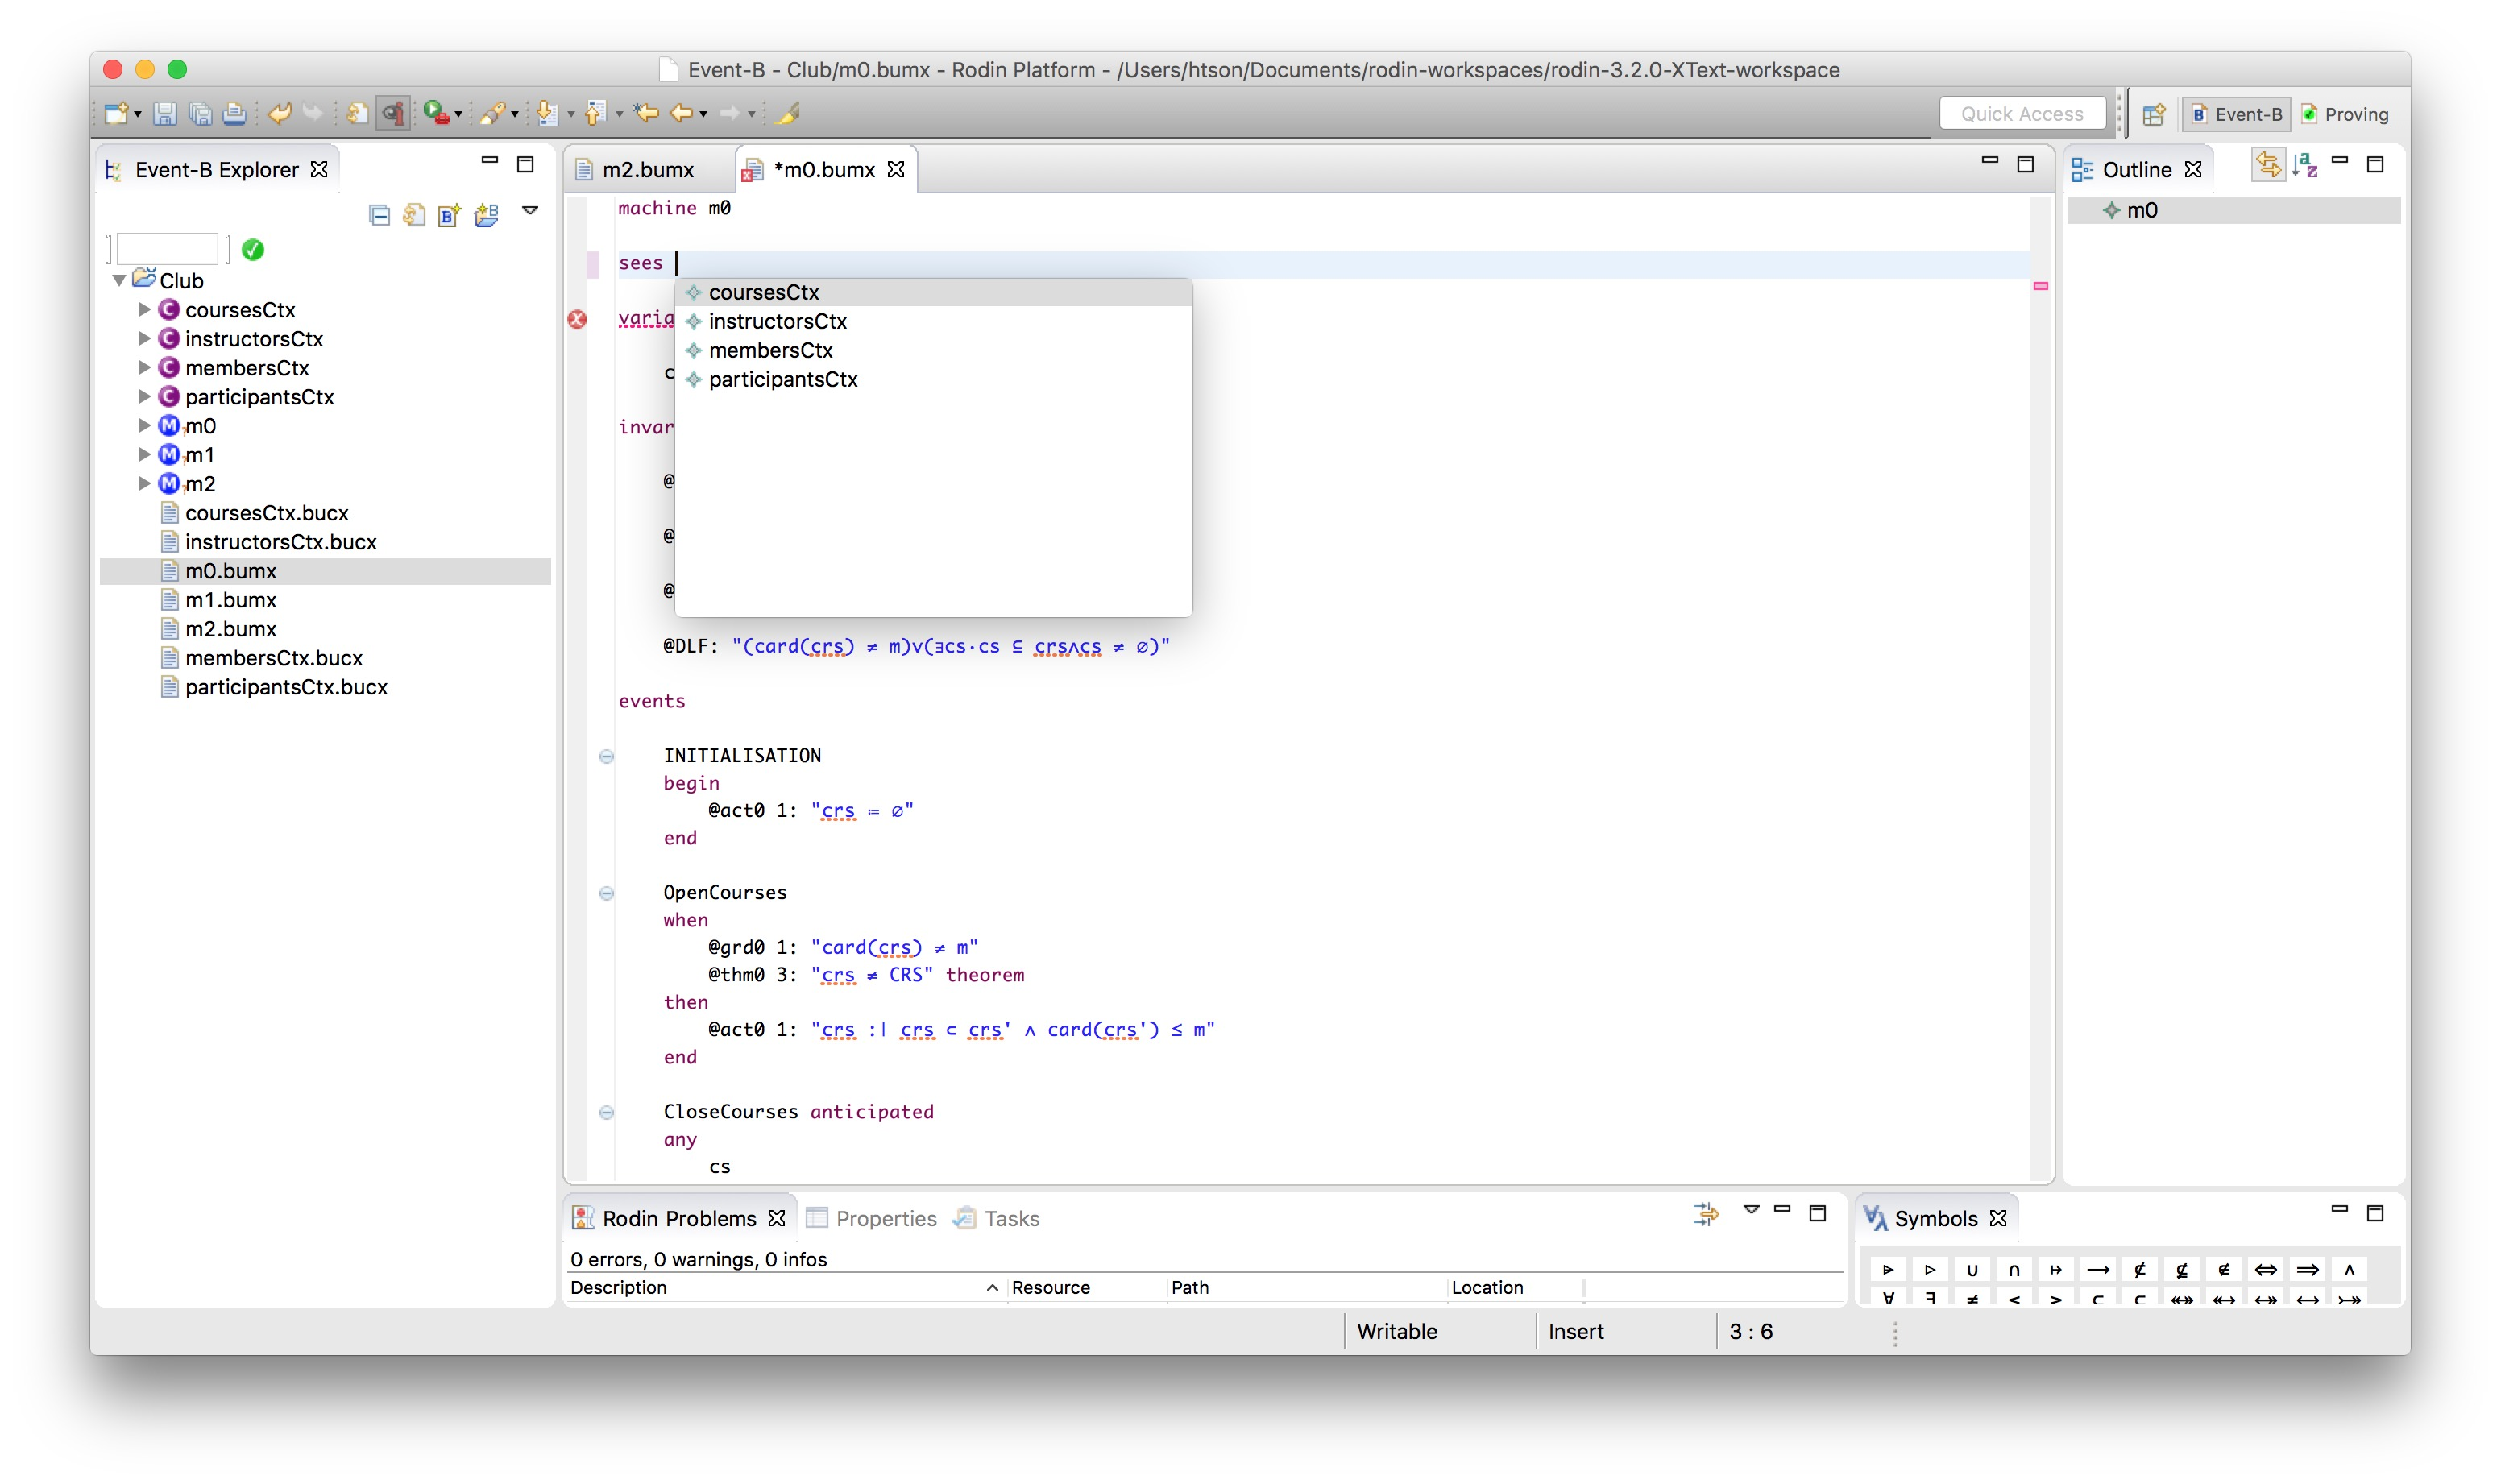
\includegraphics[width=1024]{figures/SeesContentAssist}
  \else
  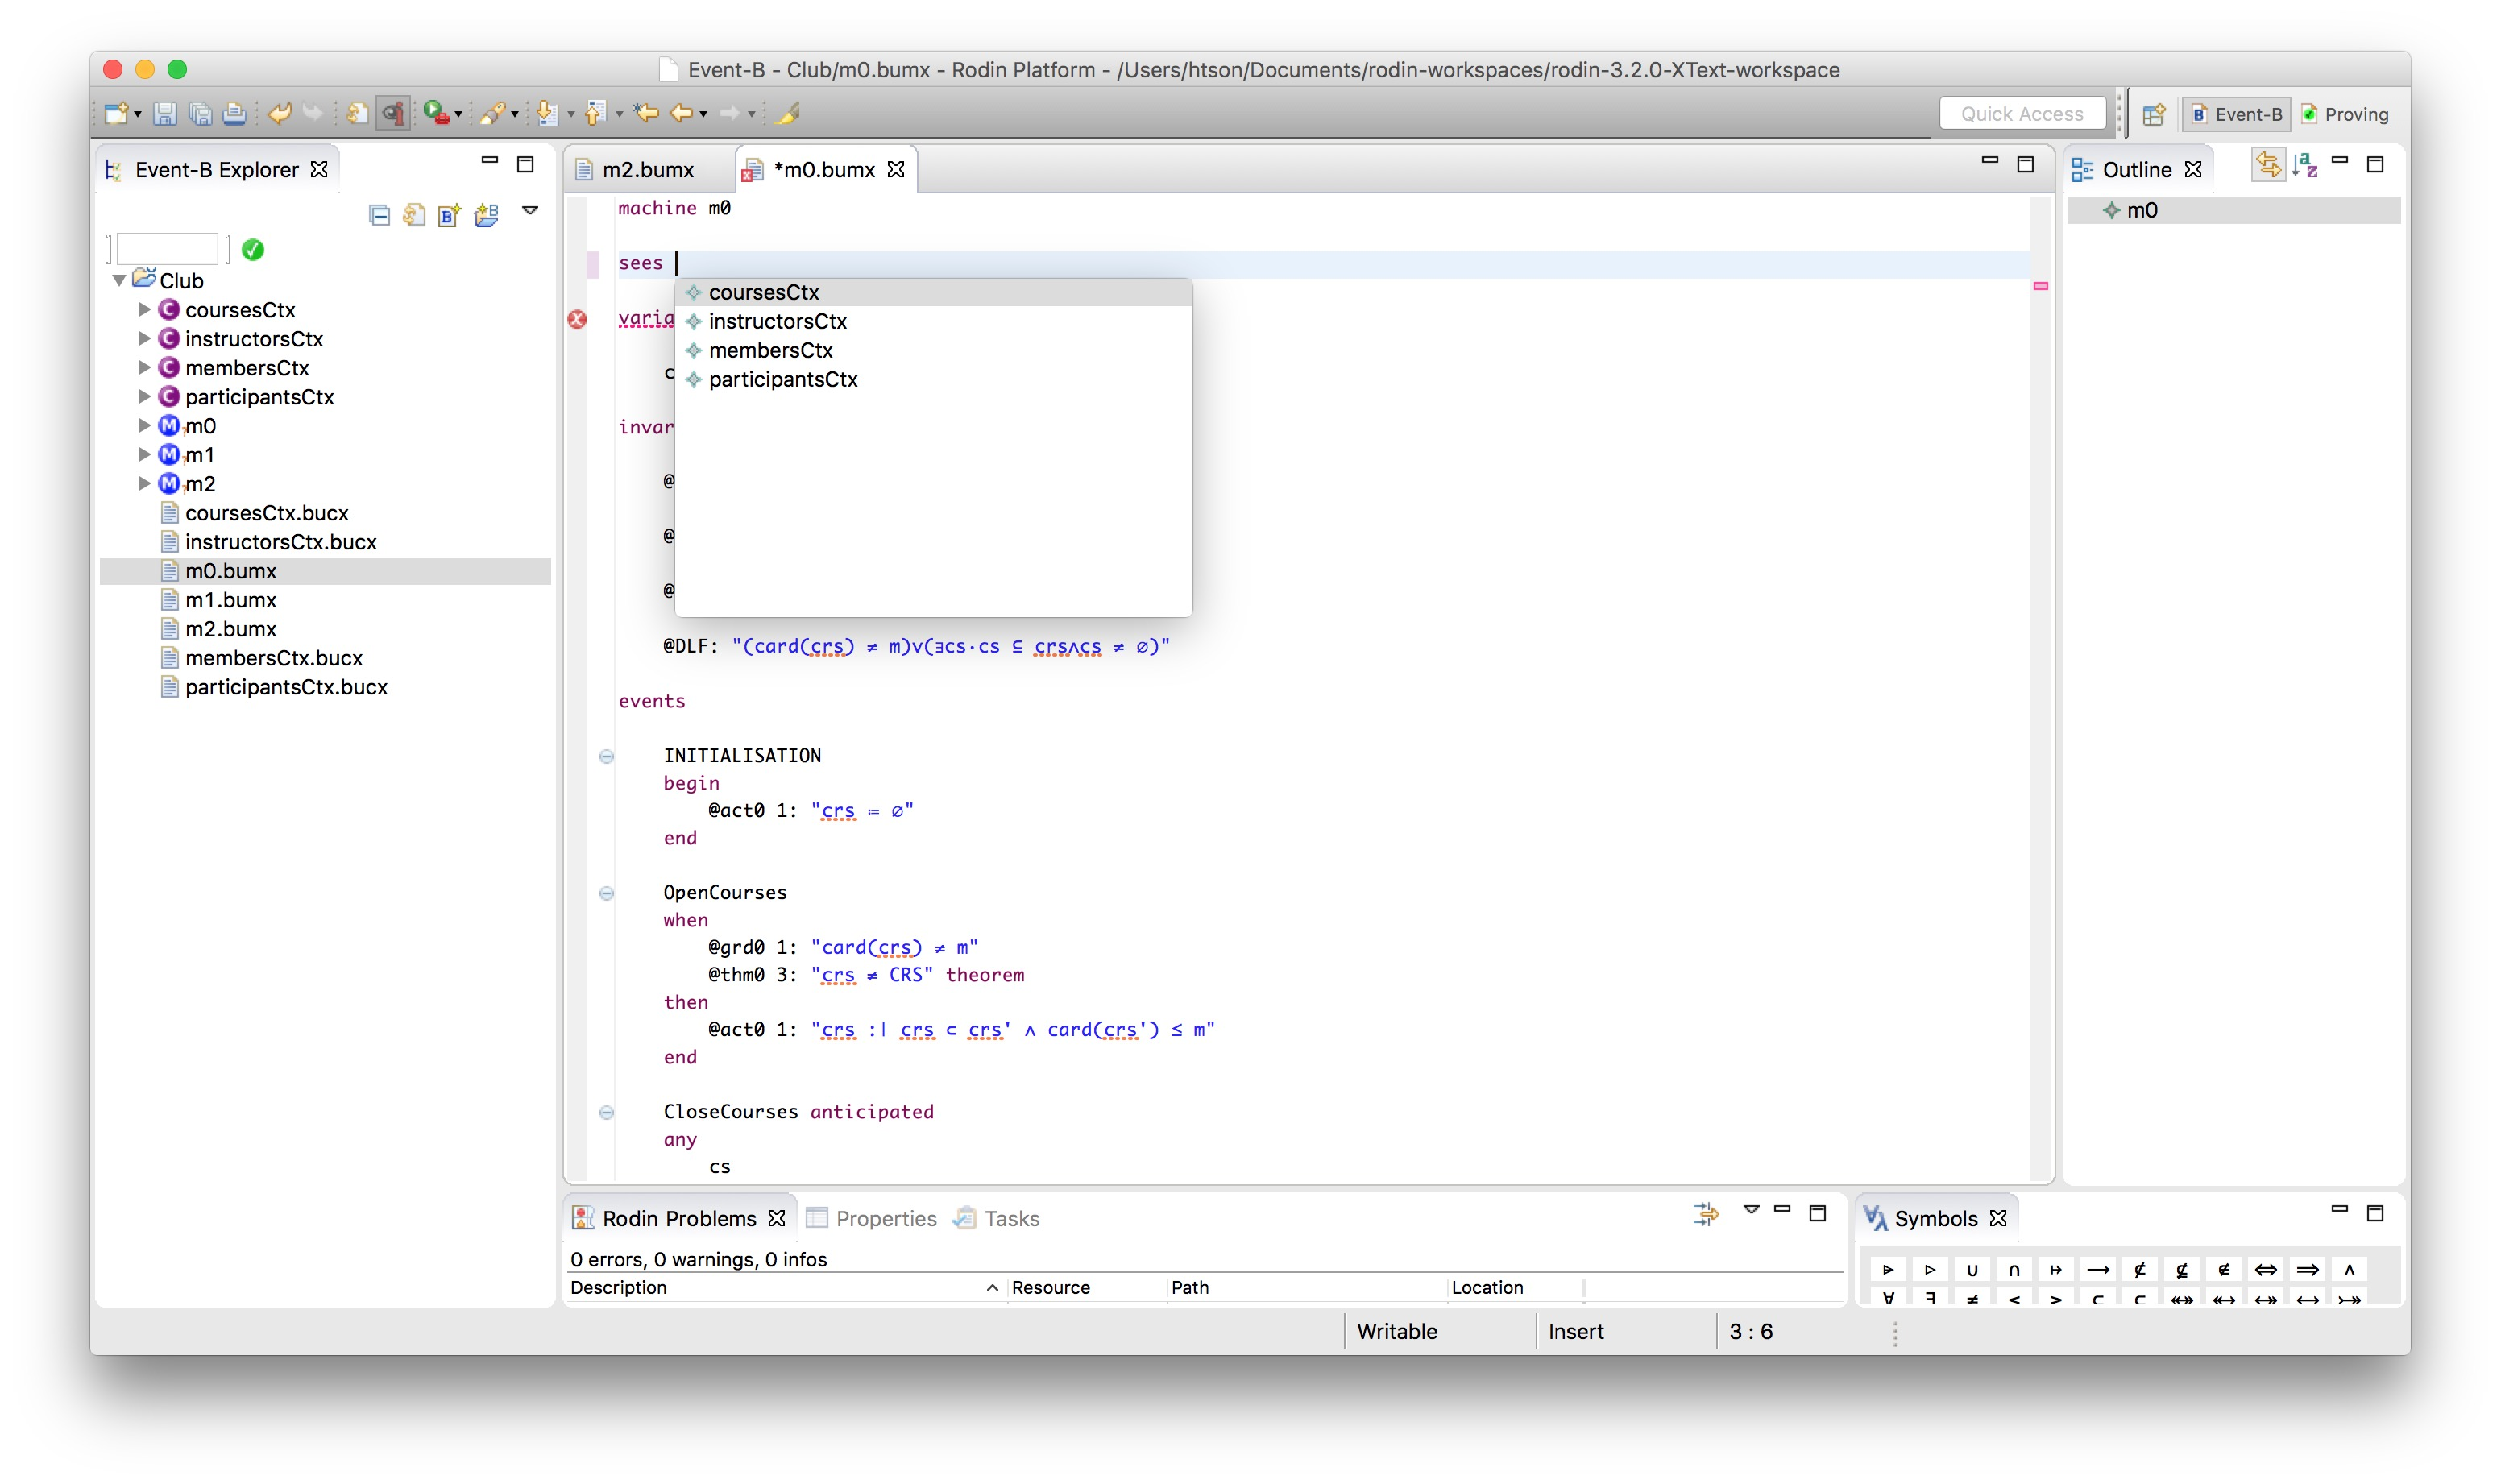
\includegraphics[width=0.9\textwidth]{figures/SeesContentAssist}
  \endif
  \caption{Content Assist for adding Sees clause}
  \label{fig:SeesContentAssist}
\end{figure}

\subsubsection{XEvent-B Formatter}
\label{sec:xevent-b-formatter}
In the XContent and XMachine editors press \texttt{Ctrl+Shift+F} on code to format it. If no selection is set then the entire source is formatted otherwise only the selection will be. 

%%% Local Variables:
%%% mode: latex
%%% TeX-master: "user_manual"
%%% End:
